\documentclass[a4paper,10pt]{article}

\usepackage[margin=2cm]{geometry}
\usepackage{graphicx}
\usepackage{amsmath}
\usepackage{array}
\usepackage{hyperref}
\usepackage[all]{hypcap}
\usepackage{listings}
\lstdefinestyle{TerminalStyle}{
  language=bash,
  basicstyle=\small\sffamily,
  numbers=left,
  numberstyle=\tiny,
  numbersep=3pt,
  frame=tb,
  columns=fullflexible,
  linewidth=0.9\linewidth,
  xleftmargin=0.1\linewidth
}
\lstdefinestyle{HtmlStyle}{
  language=html,
  basicstyle=\small\sffamily,
  numbers=left,
  numberstyle=\tiny,
  numbersep=3pt,
  frame=tb,
  columns=fullflexible,
  linewidth=0.9\linewidth,
  xleftmargin=0.1\linewidth
}
\lstdefinestyle{OutputStyle}{
  language=html,
  basicstyle=\small\sffamily,
  frame=tb,
  columns=fullflexible,
  linewidth=0.9\linewidth,
  xleftmargin=0.1\linewidth
}

\setlength{\parindent}{0pt}
\setlength{\parskip}{1ex plus 0.5ex minus 0.2ex}
\title{
\includegraphics[width=12cm]{Eeufeeslogo.jpg} \\
       Department of Computer Science \\
       University of Pretoria \\
       \vspace{0.5cm}
       Software Engineering\\
       COS301 MiniProject \\
       \vspace{0.5cm}
       \begin{large} \textbf{Navigation}\\ NavUP\end{large}}

\date{} 
\author{Bondjobo, Jocelyn 	13232852 \\
	du Plooy Andries		15226183 \\
	Brijlal	Yashvir		14387744 \\
	Jones	Keanan		13036892 \\	
	Nxumalo Banele		12201911 \\
	van Schalkwyk John	14307317 \\
}

\begin{document}
\maketitle
\thispagestyle{empty}
\clearpage

\newpage
\pagenumbering{roman}
\thispagestyle{empty}
\tableofcontents
\clearpage

\newpage
\pagenumbering{arabic}

\section{Introduction}
The reasons for which the service contract will fail can be due to a few actions occuring. 
\begin{itemize}

\item Firstly, When incorrect start and end locations are sent to the Navigation system, the system will not recognise it and will not return a route. Thus the correct desired start and endpoints must be received.


\item  A second occurance can be when the GIS module does not find a route, resulting in a null being returned. The null retuns must be handles as they will invalidate cached routes.
\end{itemize}

The only time GIS will be queries is the first time every route is requested. After that first request local cache will first be queried, thus reducing networking as well as request speed.


\section{Service Contract}
		\begin{figure}[h]
		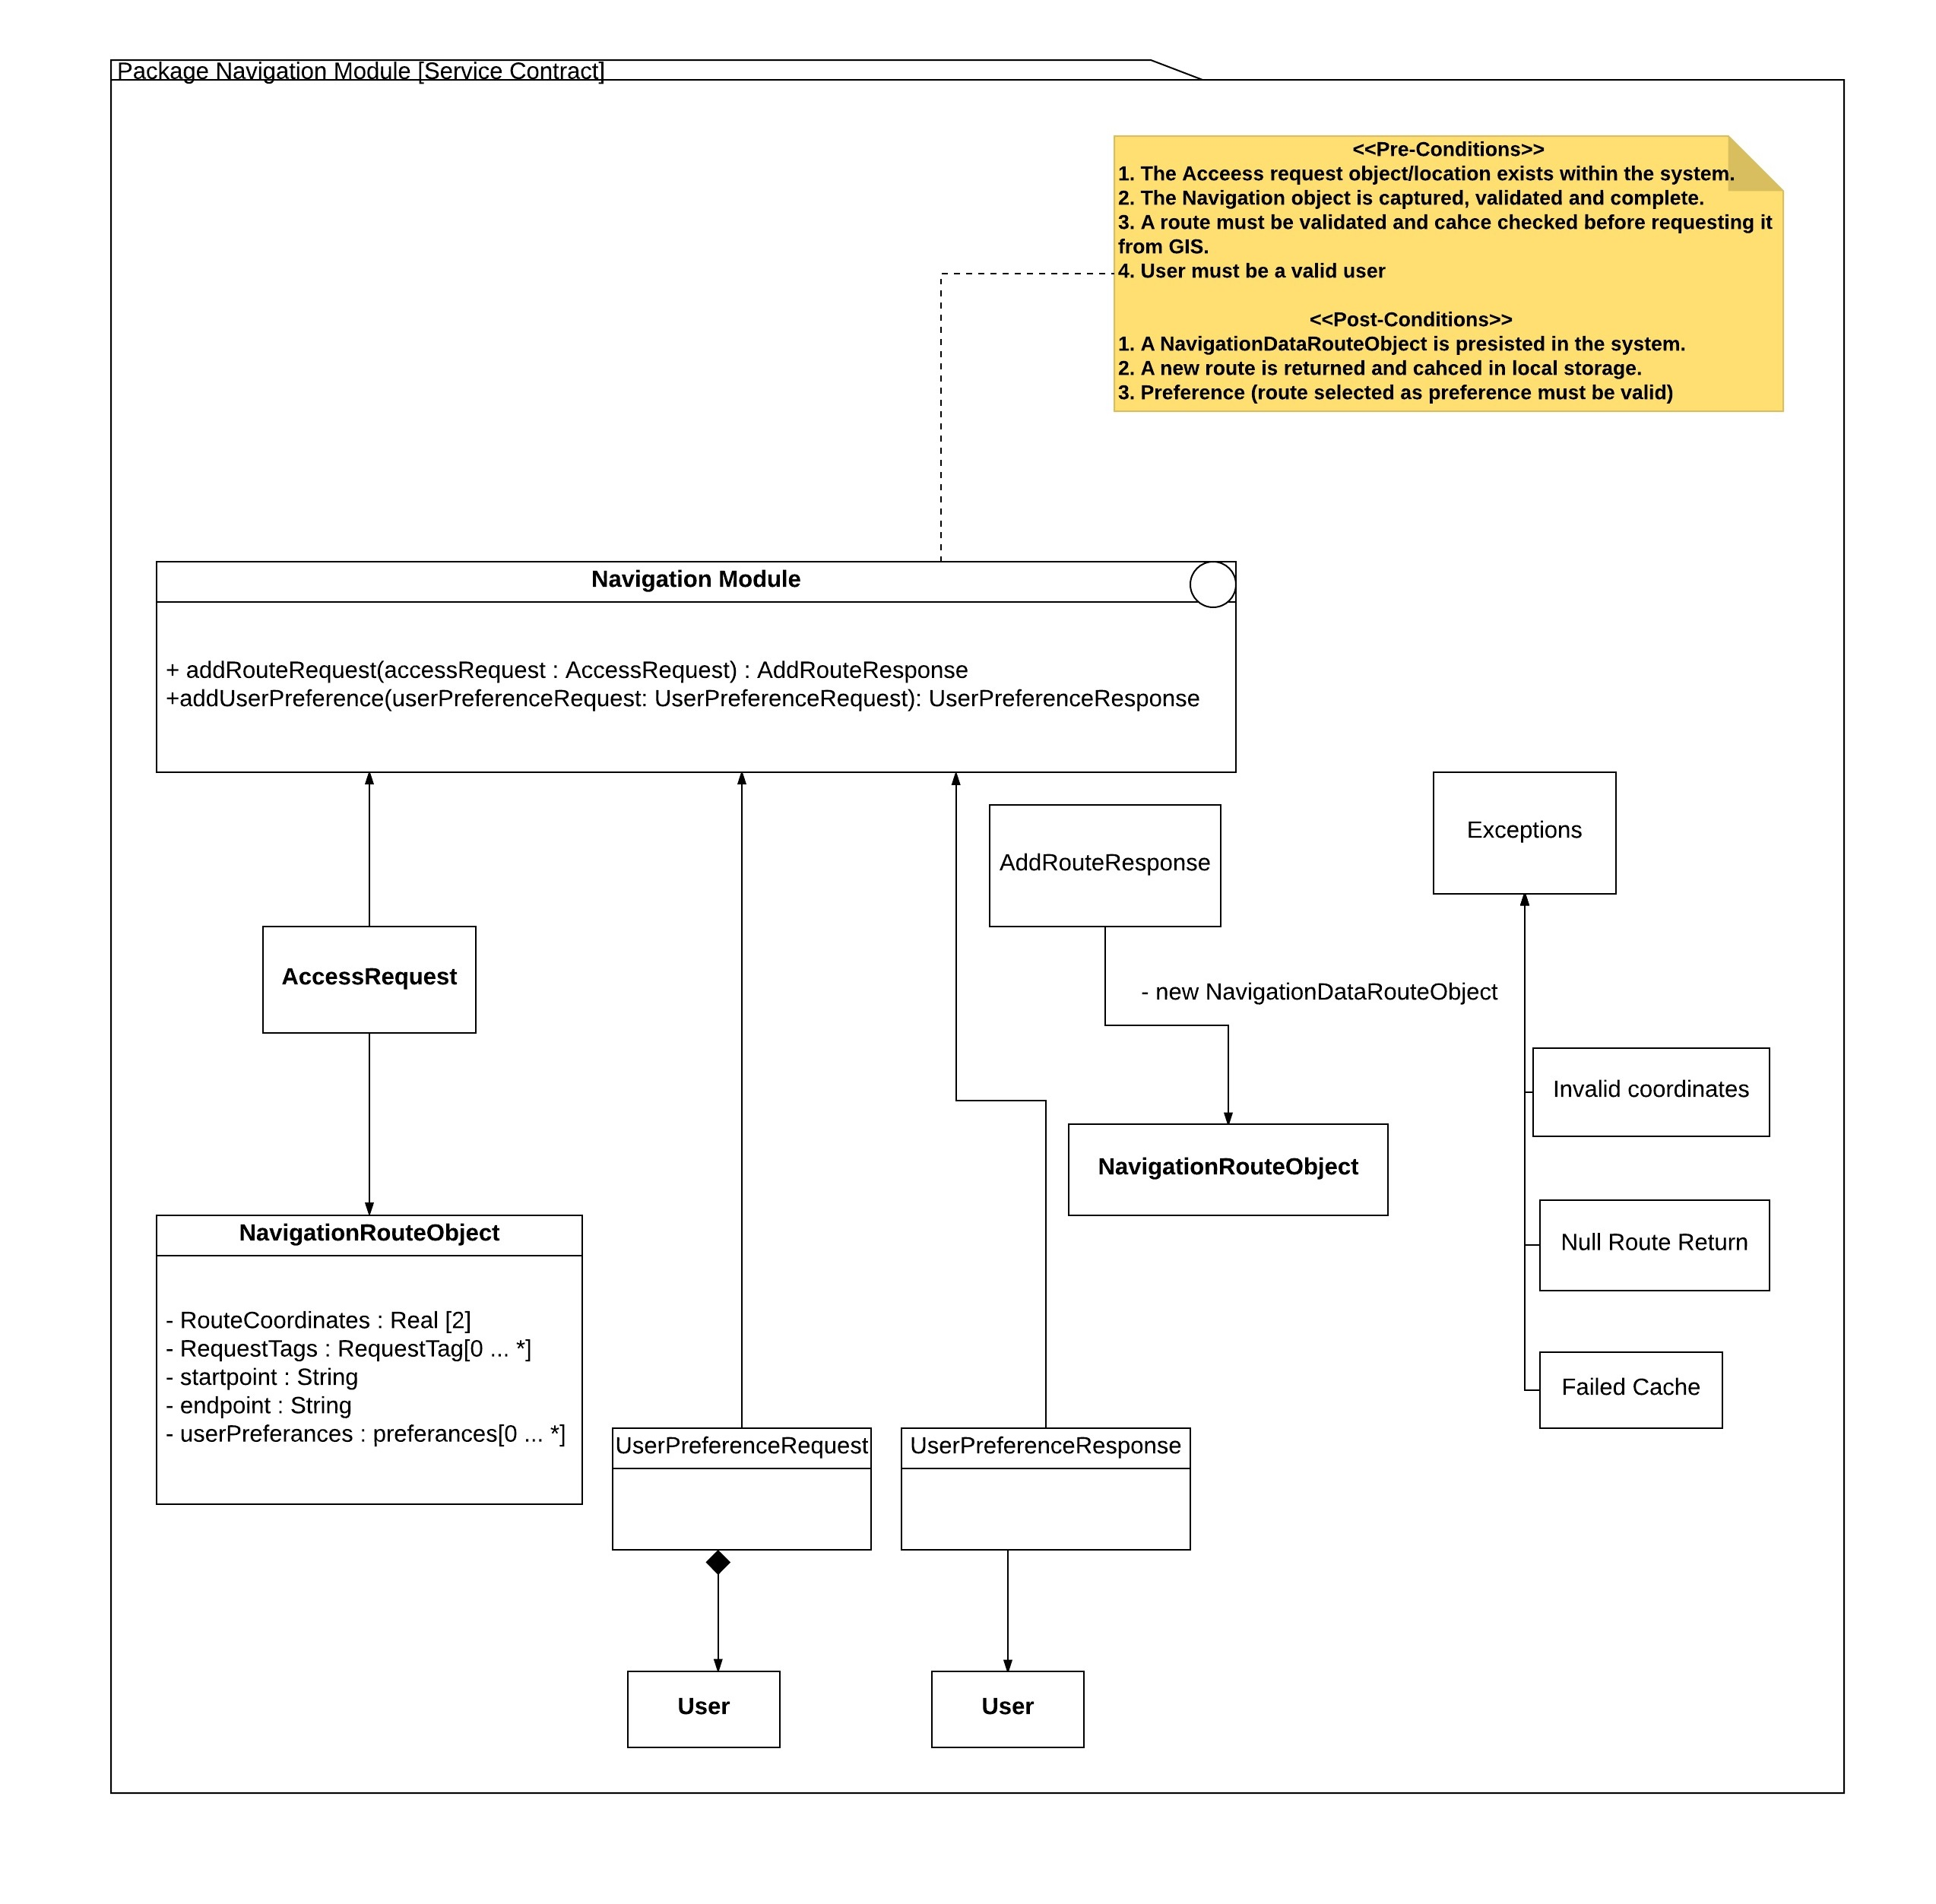
\includegraphics[scale=0.4]{Service_Contract}
		\caption{Navigation Module}
		\end{figure}

\newpage
\clearpage

\end{document}
